\chapter{Marco teórico}
\hrule  \vspace*{0.5cm}
\section{Antecedentes}
%evidencias 
%tesis referentes al tema
\subsection{Bases de datos}
Un aspecto clave del diseño de una base de datos es asegurar que el
La base de datos contiene solo valores de datos válidos consistentes con
semántica de la base de datos incluso en presencia de:
\begin{itemize}
    \item Inserciones
    \item Eliminaciones
    \item Actualizaciones
\end{itemize}
Las restricciones simplifican las aplicaciones del sistema de base de datos
realizar comprobaciones para garantizar la validez de los datos y
consistencia.\\
Esta verificación centralizada también es más confiable ya que la aplicación puede no realizar una o más de las comprobaciones.

Una base de datos solo debe contener datos válidos y consistentes
en todo momento con la posible excepción en medio de
actualizaciones \cite{gehani1990introduction}.
Algunos tipos de validez de datos se pueden garantizar mediante SQL
limitaciones.
Ejemplos:
\begin{itemize}
    \item Los estados se identifican utilizando sus abreviaturas de dos letras.
    \item Los valores deben estar dentro de un rango específico.
    \item Los campos de datos son obligatorios y no se pueden omitir.
    \item Los valores de una columna deben ser únicos.
\end{itemize}
Ejemplos de restricciones complejas de bases de datos:
\begin{itemize}
    \item Las abreviaturas de estado de 2 letras representan abreviaturas de estado válidas.
    \item Los códigos postales representan códigos postales válidos y coinciden con las direcciones especificadas.
\end{itemize}
\subsection{Introducción a Base de datos basada en grafos}
Un gráfico es una estructura de datos compuesta por aristas y vértices. La tecnología de base de datos de gráficos es una herramienta eficaz para modelar
datos cuando un enfoque en la relación entre entidades es una fuerza impulsora en el diseño de un modelo de datos.El Modelado de objetos y las relaciones entre ellos significan que casi cualquier cosa se puede representar en un gráfico correspondienteen un gráfico común.
El tipo admitido por la mayoría de los sistemas es el gráfico de propiedades. Los gráficos de propiedades son gráficos múltiples atribuidos, etiquetados y dirigidos \cite{miller2013graph}.

\vfill
\textbf{Ejemplo de BD basada en grafos}
\vfill

\begin{figure}[H]
    \centering
    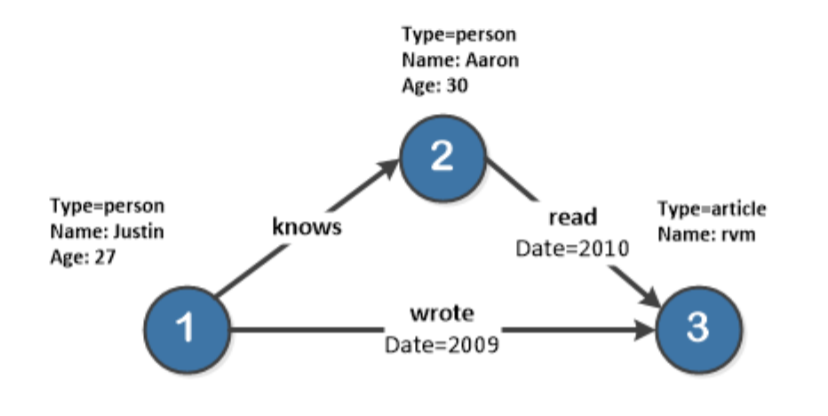
\includegraphics[scale=0.7]{Graficos/ejempbd.png}
    \caption{Ejemplo de gráfico de BDBG  Fuente: \cite{miller2013graph}.}
    \label{fig:my_label}
\end{figure}
A pesar de las limitaciones involucradas en el uso de un esquema, existen muchos beneficios, algunos de los cuales superan las restricciones implícitas en
el RDBMS. Estas bases de datos están bien respaldadas por sus respectivos proveedores, están probadas en batalla y sus las fortalezas / limitaciones son bien conocidas, tienen un lenguaje de consulta común (SQL), hay una amplia reserva de talentos de capacitados profesionales a los que recurrir, y estas plataformas están muy bien documentadas. Por el contrario, las bases de datos de gráficos se enfrentan a una conjunto de desafíos inherentes a su diseño.
\begin{figure}[H]
    \centering
    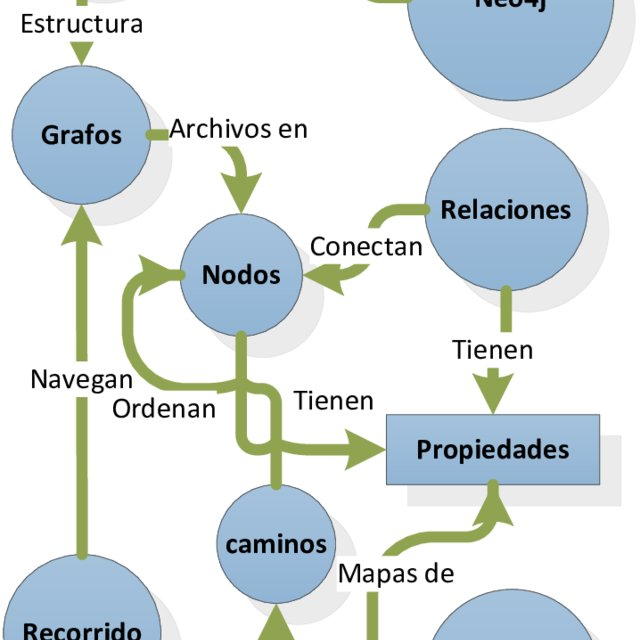
\includegraphics[scale=1]{Graficos/dbgrafo.jpg}
    \caption{Ejemplo de arquitectura de una BD basada en grafos. }
    \label{fig:my_label}
\end{figure}
\subsection{Aplicación de base de datos basado en grafos}
Las bases de datos gráficas realmente brillan cuando se trabaja en áreas donde la información sobre la interconectividad o la topología de datos es importante.
En tales aplicaciones, las relaciones entre los datos y los datos en sí suelen estar al mismo nivel . Muchas empresas tienen
desarrolló implementaciones internas para hacer frente a la necesidad de sistemas de bases de datos de gráficos\cite{miller2013graph}.\\
Ejemplos serían:
\begin{itemize}
    \item Open Graph de Facebook.
    \item Knowledge Graph de Google.
    \item FlockDB de Twitter.
\end{itemize}

\subsection{Introducción a Neo4j}
Aunque los gráficos se utilizan ampliamente durante el proceso de desarrollo de software, los desarrolladores tienden a olvidarse de los gráficos cuando se trata de la persistencia de datos. Intentamos ajustar los datos en tablas y columnas relacionales, y para normalizar y renormalizar
su estructura hasta que se vea completamente diferente de lo que está tratando de representar.
Una lista de control de acceso es un ejemplo. Este es un problema resuelto una y otra vez nuevamente en muchas aplicaciones empresariales. Por lo general, tendría tablas para usuarios, roles y recursos. Luego, tendría tablas de muchos a muchos para asignar usuarios a roles y roles a los recursos. Al final, tendrías al menos cinco tablas relacionales para representar un estructura de datos simple, que en realidad es un gráfico. Entonces usarías un objeto relacional herramienta de mapeo (ORM) para mapear estos datos a su modelo de objeto, que también es un gráfico.\\
¿No sería bueno si pudiera representar los datos en su forma natural, haciendo
mapeos más intuitivos y omitiendo el proceso repetido de "traducir" los datos
hacia y desde un motor de almacenamiento?.\\
Gracias a las bases de datos de gráficos, puede hacerlo. Bases de datos de gráficos utilizar el modelo de gráfico para almacenar datos como un gráfico, con una estructura que consta de vértices y bordes, las dos entidades utilizadas para modelar cualquier gráfico.
Además, puede utilizar todos los algoritmos de la larga historia de la teoría de grafos para resolver problemas de gráficos de manera más eficiente y en menos tiempo que usando consultas de bases de datos relacionales. \cite{vukotic2015neo4j}. 
\subsection{Graficar datos en Neo4j}
Neo4j almacena datos como vértices y bordes o, en terminología de Neo4j, nodos y relaciones. Los usuarios se representarán como nodos y las amistades se representarán como relaciones entre los nodos de usuarios. Si echa otro vistazo a la red social en la Figura \ref{fig:tiempos}, verá que no representa más que un gráfico, con los usuarios como nodos y las friendship como relaciones.
Existe una diferencia clave entre las bases de datos relacionales y Neo4j, que
se encuentran de inmediato: consulta de datos. No hay tablas ni columnas en Neo4j, tampoco hay comandos de selección y combinación basados en SQL. Entonces, ¿cómo se consulta un base de datos de gráficos?
Todos los gráficos de bases de datos, toma un poderoso concepto matemático que denota que la respuesta no es escribir una función MapReduce distribuida. Neo4j, lo muestra como teoría de grafos y lo usa como un motor poderoso y eficiente para consultar datos. Este concepto es el gráfico transversal y es una de las herramientas principales que hace que Neo4j sea tan poderoso para tratar con gráfico de datos \cite{vukotic2015neo4j}.
\begin{figure}[H]
    \centering
    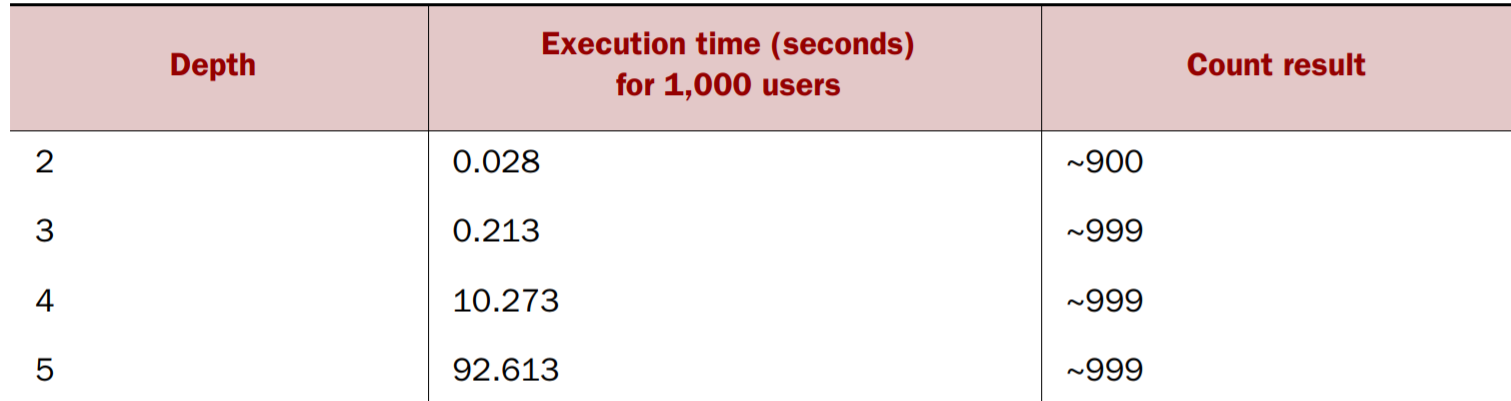
\includegraphics[scale=0.4]{Graficos/ppp.png}
    \caption{Tiempos de ejecución para múltiples consultas de combinación usando un motor de base de datos MySQL en un conjunto de datos de 1.000 usuarios}
    \label{fig:tiempos}
\end{figure}
\subsection{Neo4j en el espacio NoSQL}
Desde el comienzo del software de computadora y los datos que las aplicaciones han tenido que tratar con ha crecido enormemente en complejidad. La complejidad de los datos incluye no sólo su tamaño, también su interconexión, su estructura en constante cambio y el acceso concurrente a los datos.
Con todos estos aspectos del cambio de datos, se ha reconocido que las bases de datos relacionales, que durante mucho tiempo han sido el estándar de facto para el almacenamiento de datos, no son las más adecuadas para todos los problemas que requieren los datos cada vez más complejos. Como resultado, se ha creado una serie de nuevas tecnologías de almacenamiento, con el objetivo común de resolver
los problemas en los que las bases de datos relacionales no son buenas. Todas estas nuevas tecnologías de almacenamiento caen bajo el término general NoSQL.\\
Aunque el nombre NoSQL se atascó, no refleja con precisión la naturaleza
del movimiento, dando la impresión (errónea) de que va en contra de SQL como concepto. Un mejor nombre probablemente sería el de bases de datos no relacionales, ya que el relacional y paradigma no relacional fue el tema de discusión, mientras que SQL es sólo un lenguaje utilizado con tecnologías relacionales.
El movimiento NoSQL nació como un reconocimiento de que las nuevas tecnologías necesitaban para hacer frente a los cambios de datos. Neo4j, y las bases de datos de grafos en general, son parte del movimiento NoSQL, junto con una gran cantidad de almacenamiento más o menos relacionado con las tecnologías.
Con los rápidos desarrollos en el espacio NoSQL, su creciente popularidad y la enorme cantidad de diferentes soluciones y tecnologías para elegir, cualquiera que sea nuevo en el mundo NoSQL enfrenta muchas opciones al seleccionar la tecnología adecuada \cite{vukotic2015neo4j}. 
\subsection{Neo4j: la base de datos compatible con ACID}
La gestión de transacciones ha sido un tema de conversación destacado en las discusiones sobre las tecnologías NoSQL desde que comenzaron a ganar popularidad. Negociar atributos transaccionales para un mayor rendimiento y escalabilidad ha sido un enfoque común en tecnologías no relacionales que apuntan a big data. Algunos (como BigTable, Cassandra y CouchDB) optó por compensar la coherencia, permitiendo a los clientes leer datos obsoletos en algunos casos en un sistema distribuido (consistencia eventual). En las tiendas de valores-clave que se concentraban en el rendimiento de lectura (como Memcached), la durabilidad de los datos no generaba mucho interés. Del mismo modo, la atomicidad a nivel de una sola operación, sin la posibilidad de
envolver múltiples operaciones de bases de datos dentro de una sola transacción, es típico de las bases de datos orientadas a documentos.
Si bien cada uno de los enfoques mencionados aquí son válidos en casos de uso específicos (como el almacenamiento en caché, altos volúmenes de lectura de datos, alta carga y simultaneidad), la falta de manejo de transacciones basado en ACID suele ser el primer obstáculo cuando se trata de introducir bases de datos no relacionales a cualquier empresa o entorno corporativo. Aunque ellos
fueron ideados hace mucho tiempo para bases de datos relacionales, los atributos de transacción aún se reproducen una parte importante y fundamental en muchos casos prácticos de uso. Por tanto, Neo4j ha adoptado un enfoque diferente \cite{vukotic2015neo4j}.
